\section{Fundamento teórico}

Para comenzar se deben establecer unos parámetros para con la pala, ya que lo más básico de este trabajo empieza por determinar los efectos que produce el twisting en nuestra obtención de energía.

Es por ello que se determina que la pala de la turbina eólica es un trapecio cuya representación simplificada la vemos en la figura \ref{fig:pala_simp}

\begin{figure}[H]
    \centering
    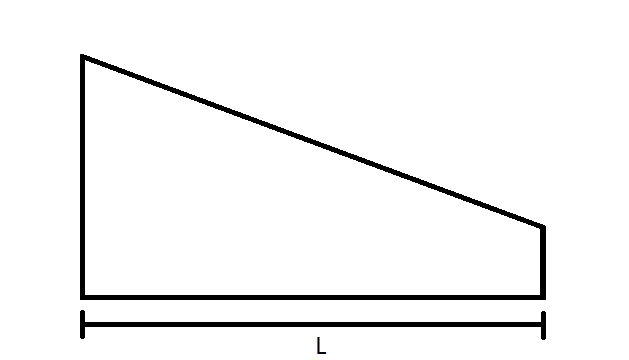
\includegraphics[width=0.7\textwidth]{images/pala turbina paint.png}
    \caption{Representación pala turbina eólica}
    \label{fig:pala_simp}
\end{figure}


Lo siguiente que se debe hacer es dividir la pala de la figura \ref{fig:pala_simp} en un número de fragmentos de igual largo, como se puede observar en la figura \ref{fig:pala_dividida}.
    
    \begin{figure}[H]
    \centering
    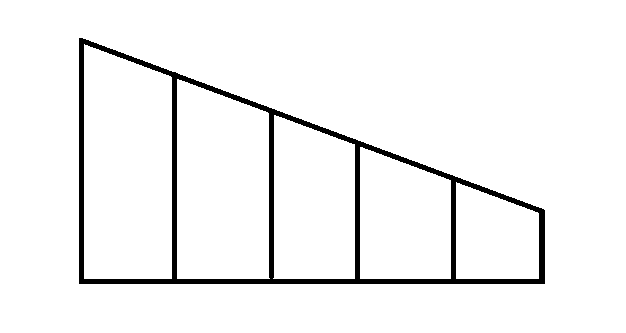
\includegraphics[width=0.7\textwidth]{images/pala dividida.png}
    \caption{Representación pala turbina eólica en fragmentos}
    \label{fig:pala_dividida}
\end{figure}

Por simplicidad, la pala se dividirá únicamente en N fragmentos, en este caso 5. Aunque se mantenga este valor durante el trabajo y es probable que no cambie, se asociará a una variable en caso de que se quieran hacer pruebas mediante MATLAB más adelante.
    
La longitud L vista en la figura \ref{fig:pala_simp} es con la que se va a trabajar, por ello cada uno de los fragmentos de la figura \ref{fig:pala_dividida} tendrá el siguiente largo $L/N = L = 5$ ya que se dividió N número de veces.


Como se puede observar en la figura \ref{fig:pala_dividida} cada fragmento tiene una altura variable, esto se debe a la forma real de las palas, cuanto más cerca de la turbina mayor es el tamaño del fragmento. 


